\documentclass[aspectratio=1610]{beamer}
%\linespread{1.5}\selectfont

\usepackage{booktabs}
\usepackage{dcolumn}
\usepackage{float}
\usepackage{placeins}
\usepackage{lscape} 
\usepackage{tikz}
\usepackage[export]{adjustbox}
\usepackage{ragged2e}
\justifying
\usepackage{outlines}
\usepackage{amsmath}
\usepackage{booktabs}
\usepackage{float}
\usepackage{hyperref}	
\usepackage{dcolumn}
\usepackage{longtable}
\usepackage{array}
\usepackage{multirow}
\usepackage{wrapfig}
\usepackage{float}
\usepackage{colortbl}
\usepackage{pdflscape}
\usepackage{tabu}
\usepackage{threeparttable}
\usepackage{caption}
%\captionsetup{font=footnotesize}
\usepackage{subcaption}
\usepackage{threeparttable}
\usepackage[normalem]{ulem}
\usepackage{makecell}
\usepackage{xcolor}
%\usepackage{caption}
%\captionsetup{labelformat=empty}
\usepackage{appendixnumberbeamer}
\DeclareUnicodeCharacter{2212}{-}

\usepackage[backend = biber, style=authoryear, sorting = nty, maxnames=1]{biblatex}

\addbibresource{../../../citations_sesmarias.bib}

% \addbibresource[glob]{~/OneDrive-UniversityofIllinois-Urbana/Research/Writing/Sesmarias/citations_sesmarias.bib}
\renewcommand*{\nameyeardelim}{\addcomma\space}

\usepackage{setspace}

\DeclareUnicodeCharacter{0301}{\'{e}}
\usepackage{graphicx}

\newcommand{\tinytable}[1]{\textcolor{black}{\tiny \input{#1}}}

\graphicspath{{~/OneDrive-UniversityofIllinois-Urbana/Research/Writing/Sesmarias/00. Pictures/}}

\beamertemplatenavigationsymbolsempty

%Information to be included in the title page:
\title{Sesmaria Land Grants and the Origins of Brazilian Inequality}
\author{Vinicius Okada da Silva}
\institute{University of Illinois at Urbana-Champaign}
\date{}

\setbeamertemplate{footline}[frame number]

\begin{document}


\begin{frame}[plain, noframenumbering]
	\titlepage
\end{frame}

\begin{frame}{History}
    \begin{outline}
        \1 Originally a medieval Portuguese Law used to grant lands to be used and developed.
        \1 First mention of it in Brazil was in 1530, and it often favored the Portuguese aristocracy \parencite{Lobb1976-mc}
            \2 It led to the development of the ``economic aristocracy of the colonial society'' and the ``principal cause of the \textit{latifundio}'' in Brazil \parencites[p.~36]{Lima2002-kd}[p.~48]{Da_Costa_Porto1979-dz}.
            \2 Officially stopped being granted in 1822, however, \textit{sesmeiro} who had owned land and had developed it would be able to retain their lands.
    \end{outline}    
\end{frame}

\begin{frame}{Research Question}
    \begin{outline}
        \1 What are the long-term economic effects of the \textit{sesmarias} land grants in Brazil?
            \2 Land inequality $\Rightarrow$ only those with financial conditions were granted \textit{sesmarias}, and were often granted large plots of land.
            \2 Income inequality $\Rightarrow$ land was wealth, fewer people with land lead to wealth accumulation by the few.
            %\2 Urban development $\Rightarrow$ .
    \end{outline}
\end{frame}

\begin{frame}{Data}
    \begin{outline}
        \1 Brazilian Censuses (1872-2010)
        \1 Location of \textit{sesmarias} from SILB.
    \end{outline}
\end{frame}

\begin{frame}{Example of Document}
    \begin{figure}
        \centering
        \begin{subfigure}[t]{0.35\textwidth}
        \centering
        \vspace{-7.4cm}
        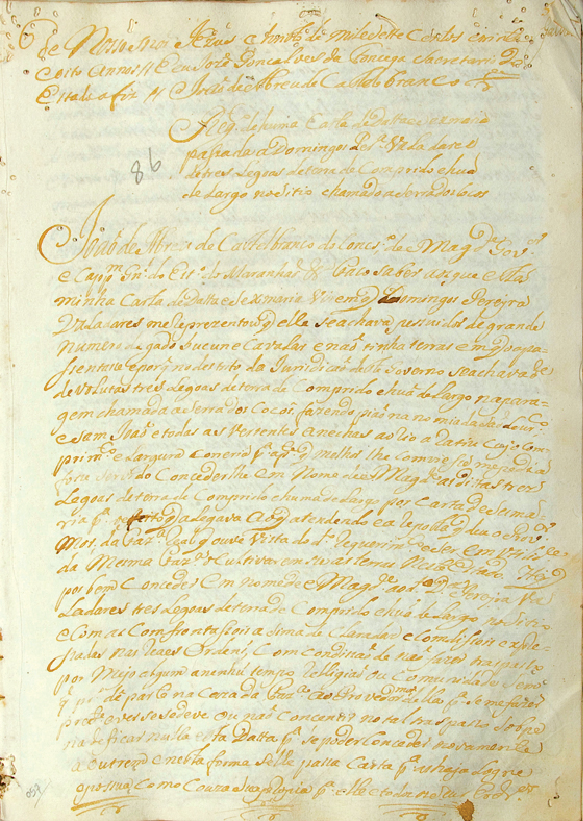
\includegraphics[width = \textwidth]
        {Pictures/0167f614a7c3b3fd38127f1545dbee7c.pdf}
        \end{subfigure}
        \hspace{0.2cm}
        \qquad\tikz[baseline=-\baselineskip]\draw[ultra thick,->] (0,4) -- ++ (1,0);\qquad
        \hspace{-0.25cm}
        \begin{subfigure}[t]{0.4\textwidth}
        \centering
        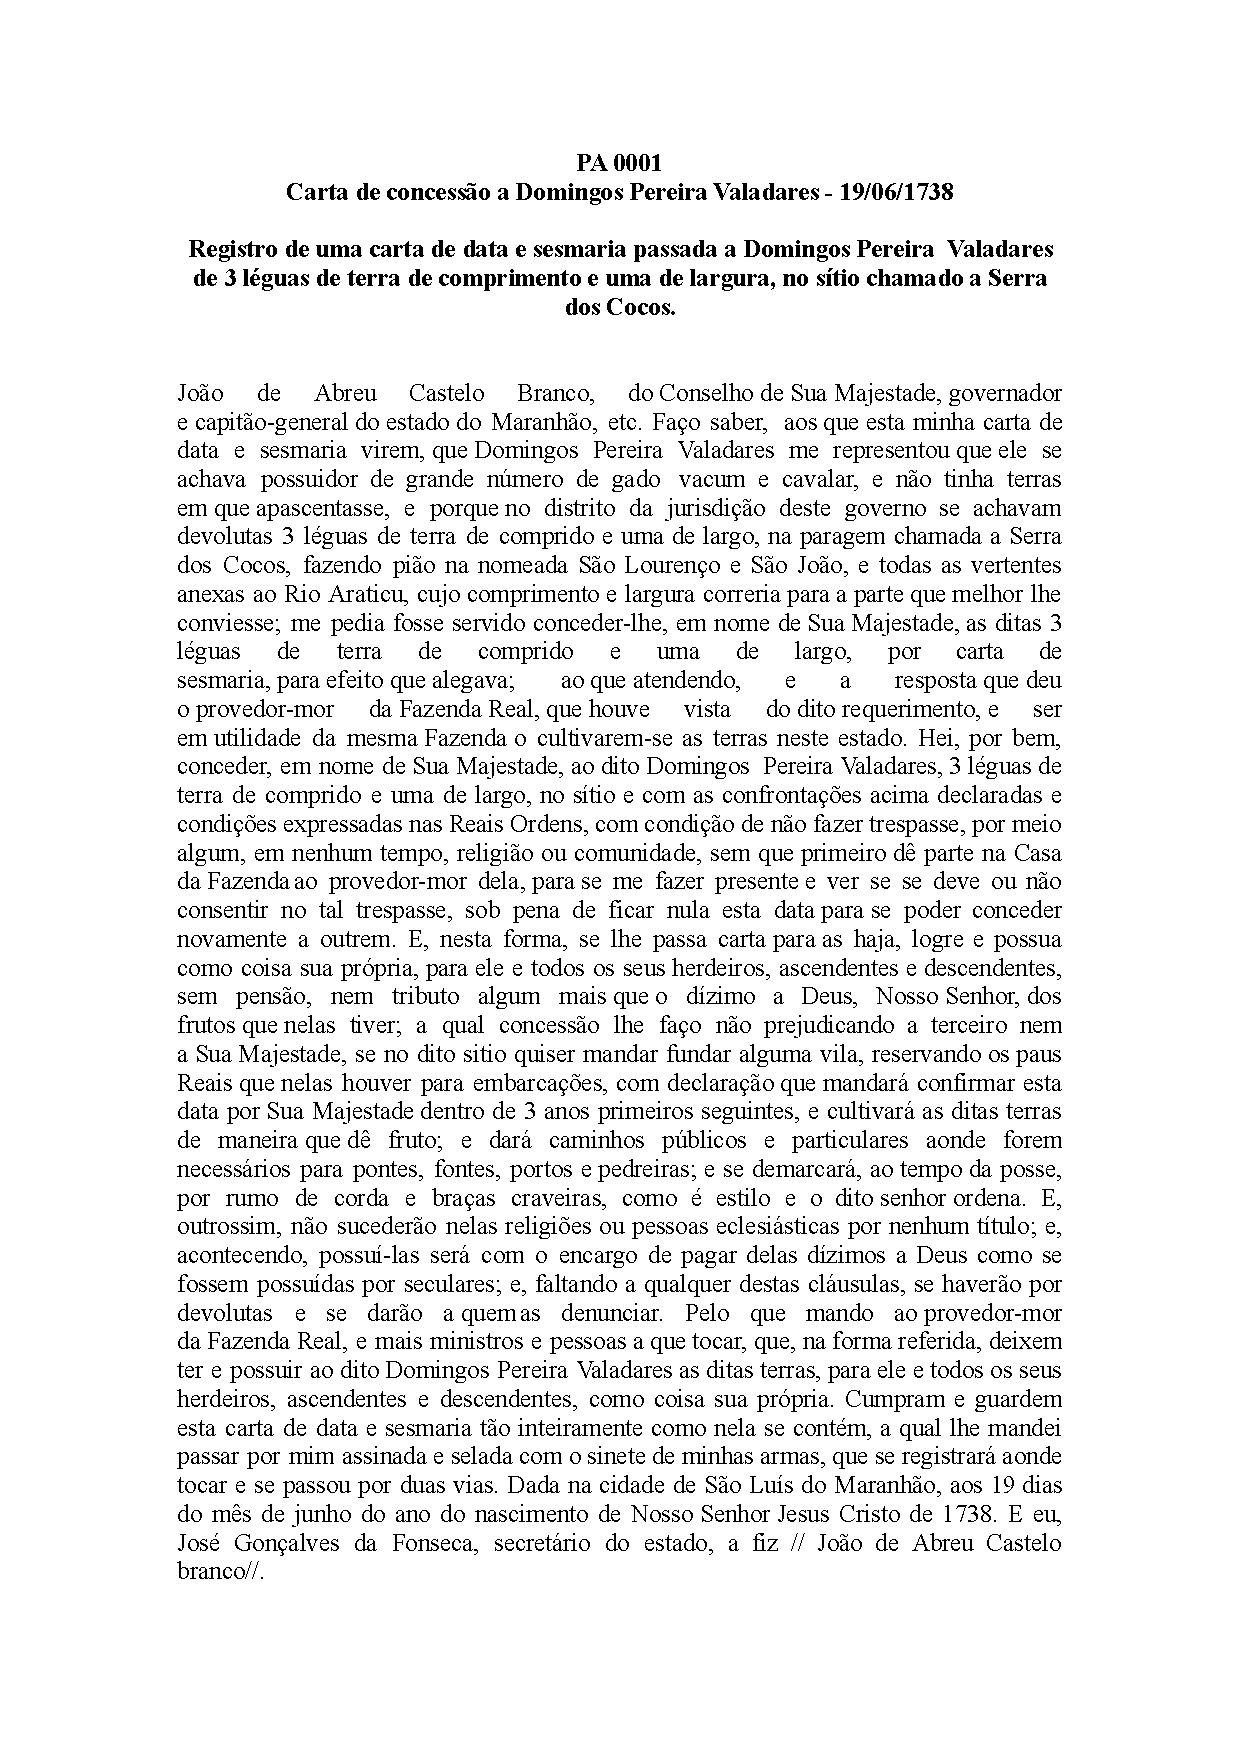
\includegraphics[page = 1, width = \textwidth]
        {Pictures/ea71ea6ac7c5ec3cefa24ded60ac6438.pdf}
        \end{subfigure}
    \end{figure}
\end{frame}


\begin{frame}{Possible Sources of Variation}
    \begin{outline}
        \1 Geographical Variation
        \1 Time Variation
        \1 Type of Settler to whom it was granted
        \1 Concessions vs. Applications
    \end{outline}
\end{frame}

\begin{frame}{Other Relevant (?) Information to Add}
    \begin{outline}
        \1 Sesmarias caused land uncertainty in colonial times as often poor people would settle, develop land, and then lose the right of the land because a richer person would claim it \parencite[p.~142]{Da_Costa_Porto1979-dz}.

    \end{outline}
\end{frame}

\begin{frame}[allowframebreaks, t]{References}
    \printbibliography
\end{frame}

\end{document}